\chapter{Các hệ thống và thuật toán liên quan}
\label{Chapter2}

\emph{Chương này giới thiệu về một số hệ thống tương tự với hệ thống chỉ đường cũng như một số thuật toán xử lí giọng nói.}

\section{Các hệ thống tương tự}

Trên thế giới, nhiều hệ thống hỗ trợ

\section{Một số hệ thống hiểu ngôn ngữ tự nhiên}

\subsection{Giới thiệu về hiểu ngôn ngữ tự nhiên}

Hiểu ngôn ngữ tự nhiên là một chủ đề của xử lý ngôn ngữ tự nhiên trong lĩnh vực trí tuệ nhân tạo. Để có thể xây dựng một chatbot hoặc trợ lý giọng nói thì điều không thể thiếu đó chính là hiểu được ngôn ngữ tự nhiên.

Bất cứ khi nào người dùng tương tác với AI bằng ngôn ngữ tự nhiên, các từ của họ cần phải được dịch thành một mô tả mà máy có thể đọc được về ý của họ.
Công cụ \ac{nlu} trước tiên phát hiện ý định của người dùng là gì (intent), sau đó trích xuất các tham số (slot) của truy vấn. Sau đó, nhà phát triển có thể sử dụng điều này để xác định hành động hoặc phản hồi thích hợp.

\subsection{Một số phương pháp hiểu ngôn ngữ tự nhiên}

\begin{itemize}
    \item Rasa \ac{nlu}
          \begin{figure}[htp]
              \centering
              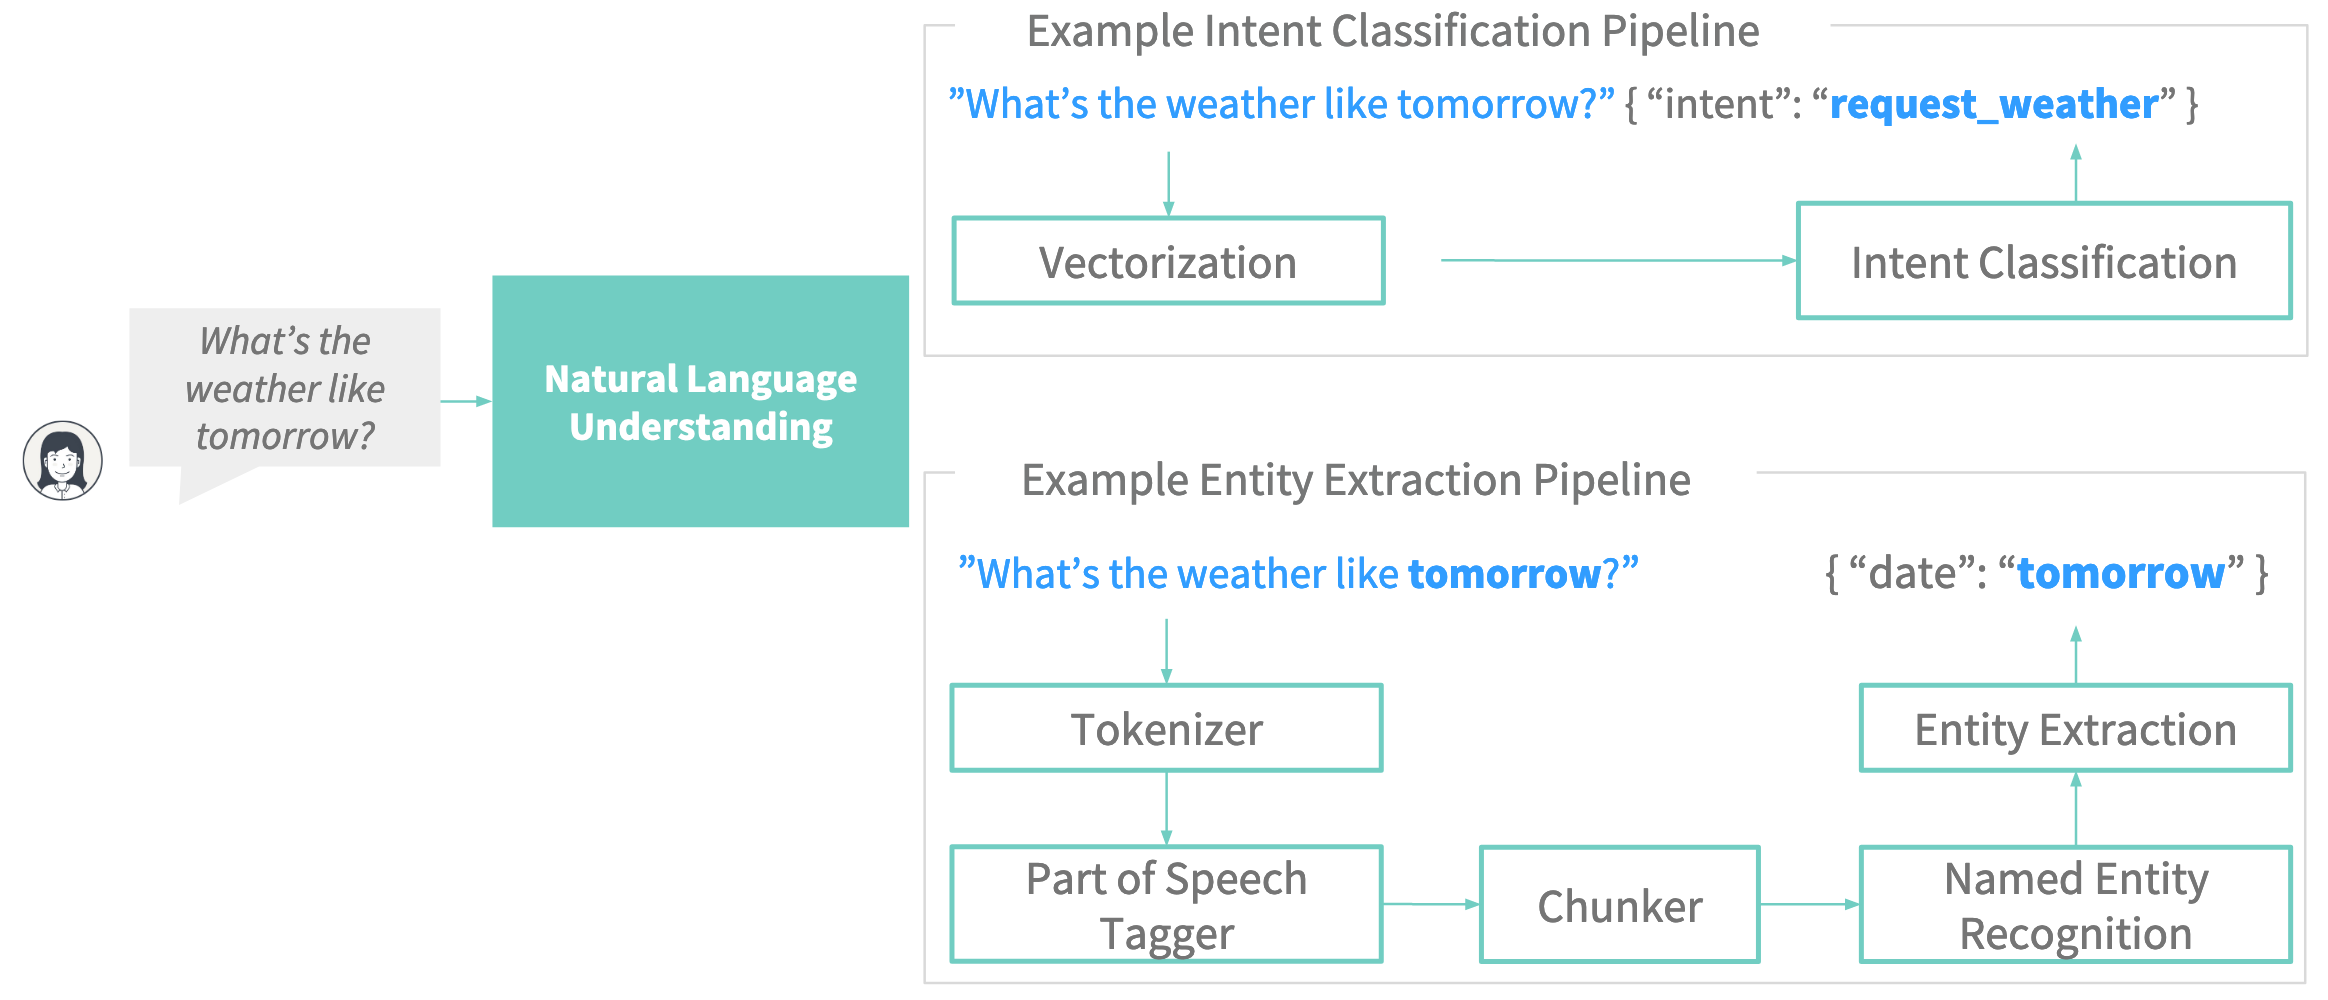
\includegraphics[width=10cm]{images/Rasa-NLU.png}
              \caption{Sơ đồ hệ thống Rasa-\ac{nlu}}
              \label{fig:rasa-nlu}
          \end{figure}
    \item Snips \ac{nlu}
          \begin{figure}[htp]
              \centering
              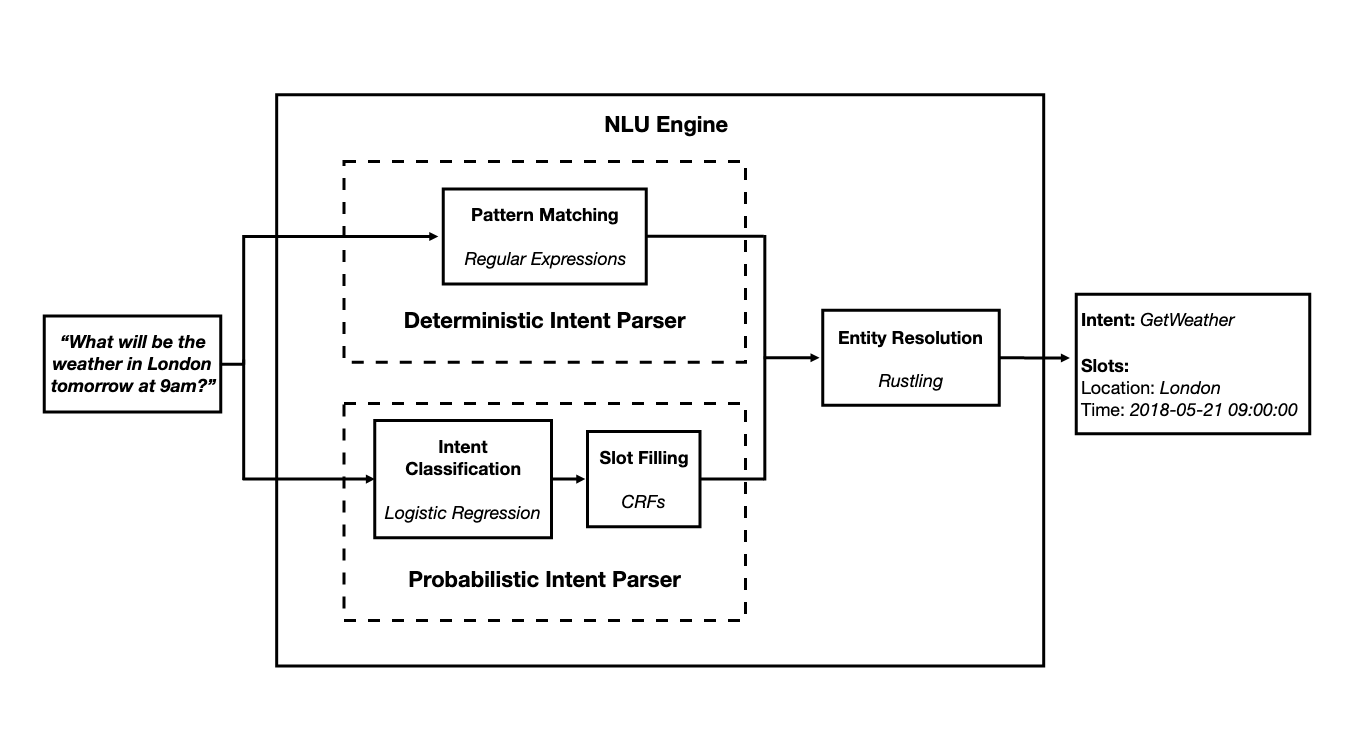
\includegraphics[width=10cm]{images/Snips-NLU.png}
              \caption{Sơ đồ hệ thống Snips-\ac{nlu}}
              \label{fig:snips-nlu}
          \end{figure}
          
          Có thể khái quát các luồng xử lý của snips-NLU \cite{snips-nlu} như sau:
          
          Hệ thống Snips-NLU (hình \ref{fig:snips-nlu}) chứa một thành phần chính, NLU Engine, bản thân nó bao gồm một số thành phần sau:
          \begin{itemize}
              \item Deterministic intent parser: Mục tiêu của trình phân tích cú pháp xác định là cung cấp độ mạnh mẽ và trải nghiệm có thể dự đoán được cho người dùng vì nó được đảm bảo đạt được 1.0 F1-Score trên các ví dụ đào tạo. Các truy vấn có trong dữ liệu huấn luyện được sử dụng để xây dựng các mẫu bao gồm tất cả các tổ hợp giá trị thực thể.
              \item Probabilistic intent parser: Trình phân tích cú pháp mục đích nhằm mục đích mở rộng phân tích cú pháp vượt ra ngoài các ví dụ đào tạo và nhận ra các biến thể không xuất hiện trong dữ liệu đào tạo. Nó cung cấp sức mạnh tổng quát hóa mà trình phân tích cú pháp xác định thiếu. Thông qua hai bước intent classification (xác định ý định) and slot filling (trích xuất thực thể).
              \item Entity resolution:
          \end{itemize}
\end{itemize}